\chapter{System Design}
This chapter discusses the system design, analysing the various aspects of the project and purpose of each component such as the visualisation, the sorting algorithms, user authentication, the server, etc.

\section{Overview}
\begin{center}
    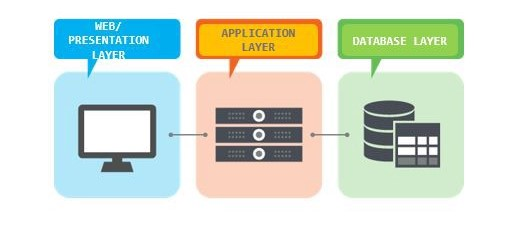
\includegraphics[width=8cm,height=3.3cm,keepaspectratio]{images/3tier}
\end{center}

This project utilises the multi-tier architecture (often referred to as n-tier architecture) platform. Multi-tier architecture or multilayered architecture is a client–server architecture in which presentation, application processing, and data management functions are physically separated. The most widespread use of multi-tier architecture is the three-tier architecture. This project consists of ... main components, all working together: The web application, which represents the presentation layer, allows users to visualise various sorting algorithms, register and login, upload and view past sorts from other users. The Flask server, which represents the logic tier, handles requests such as account registration and log in, and uploading and retrieving of sorts by users.

\begin{center}
    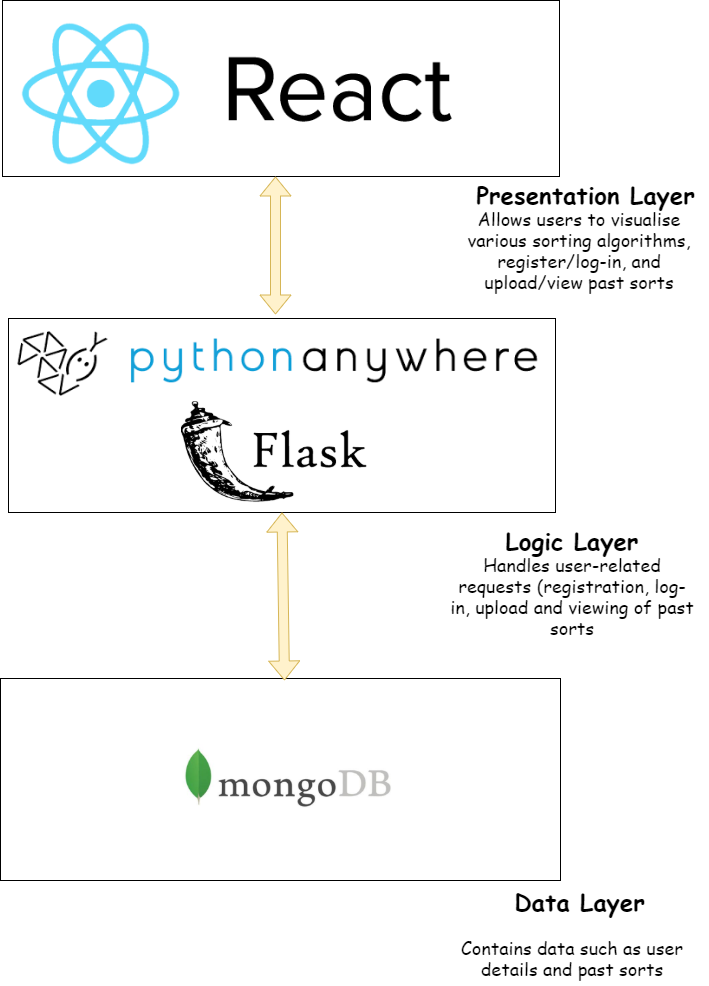
\includegraphics[width=15cm,height=15cm,keepaspectratio]{images/system_design}
\end{center}
\newpage

\section{Web Application}

\section{Flask Server}

\section{Database}
